% Options for packages loaded elsewhere
\PassOptionsToPackage{unicode}{hyperref}
\PassOptionsToPackage{hyphens}{url}
%
\documentclass[
]{article}
\usepackage{amsmath,amssymb}
\usepackage{lmodern}
\usepackage{iftex}
\ifPDFTeX
  \usepackage[T1]{fontenc}
  \usepackage[utf8]{inputenc}
  \usepackage{textcomp} % provide euro and other symbols
\else % if luatex or xetex
  \usepackage{unicode-math}
  \defaultfontfeatures{Scale=MatchLowercase}
  \defaultfontfeatures[\rmfamily]{Ligatures=TeX,Scale=1}
\fi
% Use upquote if available, for straight quotes in verbatim environments
\IfFileExists{upquote.sty}{\usepackage{upquote}}{}
\IfFileExists{microtype.sty}{% use microtype if available
  \usepackage[]{microtype}
  \UseMicrotypeSet[protrusion]{basicmath} % disable protrusion for tt fonts
}{}
\makeatletter
\@ifundefined{KOMAClassName}{% if non-KOMA class
  \IfFileExists{parskip.sty}{%
    \usepackage{parskip}
  }{% else
    \setlength{\parindent}{0pt}
    \setlength{\parskip}{6pt plus 2pt minus 1pt}}
}{% if KOMA class
  \KOMAoptions{parskip=half}}
\makeatother
\usepackage{xcolor}
\usepackage[margin=1in]{geometry}
\usepackage{graphicx}
\makeatletter
\def\maxwidth{\ifdim\Gin@nat@width>\linewidth\linewidth\else\Gin@nat@width\fi}
\def\maxheight{\ifdim\Gin@nat@height>\textheight\textheight\else\Gin@nat@height\fi}
\makeatother
% Scale images if necessary, so that they will not overflow the page
% margins by default, and it is still possible to overwrite the defaults
% using explicit options in \includegraphics[width, height, ...]{}
\setkeys{Gin}{width=\maxwidth,height=\maxheight,keepaspectratio}
% Set default figure placement to htbp
\makeatletter
\def\fps@figure{htbp}
\makeatother
\setlength{\emergencystretch}{3em} % prevent overfull lines
\providecommand{\tightlist}{%
  \setlength{\itemsep}{0pt}\setlength{\parskip}{0pt}}
\setcounter{secnumdepth}{-\maxdimen} % remove section numbering
\ifLuaTeX
  \usepackage{selnolig}  % disable illegal ligatures
\fi
\IfFileExists{bookmark.sty}{\usepackage{bookmark}}{\usepackage{hyperref}}
\IfFileExists{xurl.sty}{\usepackage{xurl}}{} % add URL line breaks if available
\urlstyle{same} % disable monospaced font for URLs
\hypersetup{
  pdftitle={Model \& Selection},
  pdfauthor={Mark D},
  hidelinks,
  pdfcreator={LaTeX via pandoc}}

\title{Model \& Selection}
\author{Mark D}
\date{2023-01-27}

\begin{document}
\maketitle

\hypertarget{project-methodology}{%
\subsection{Project methodology}\label{project-methodology}}

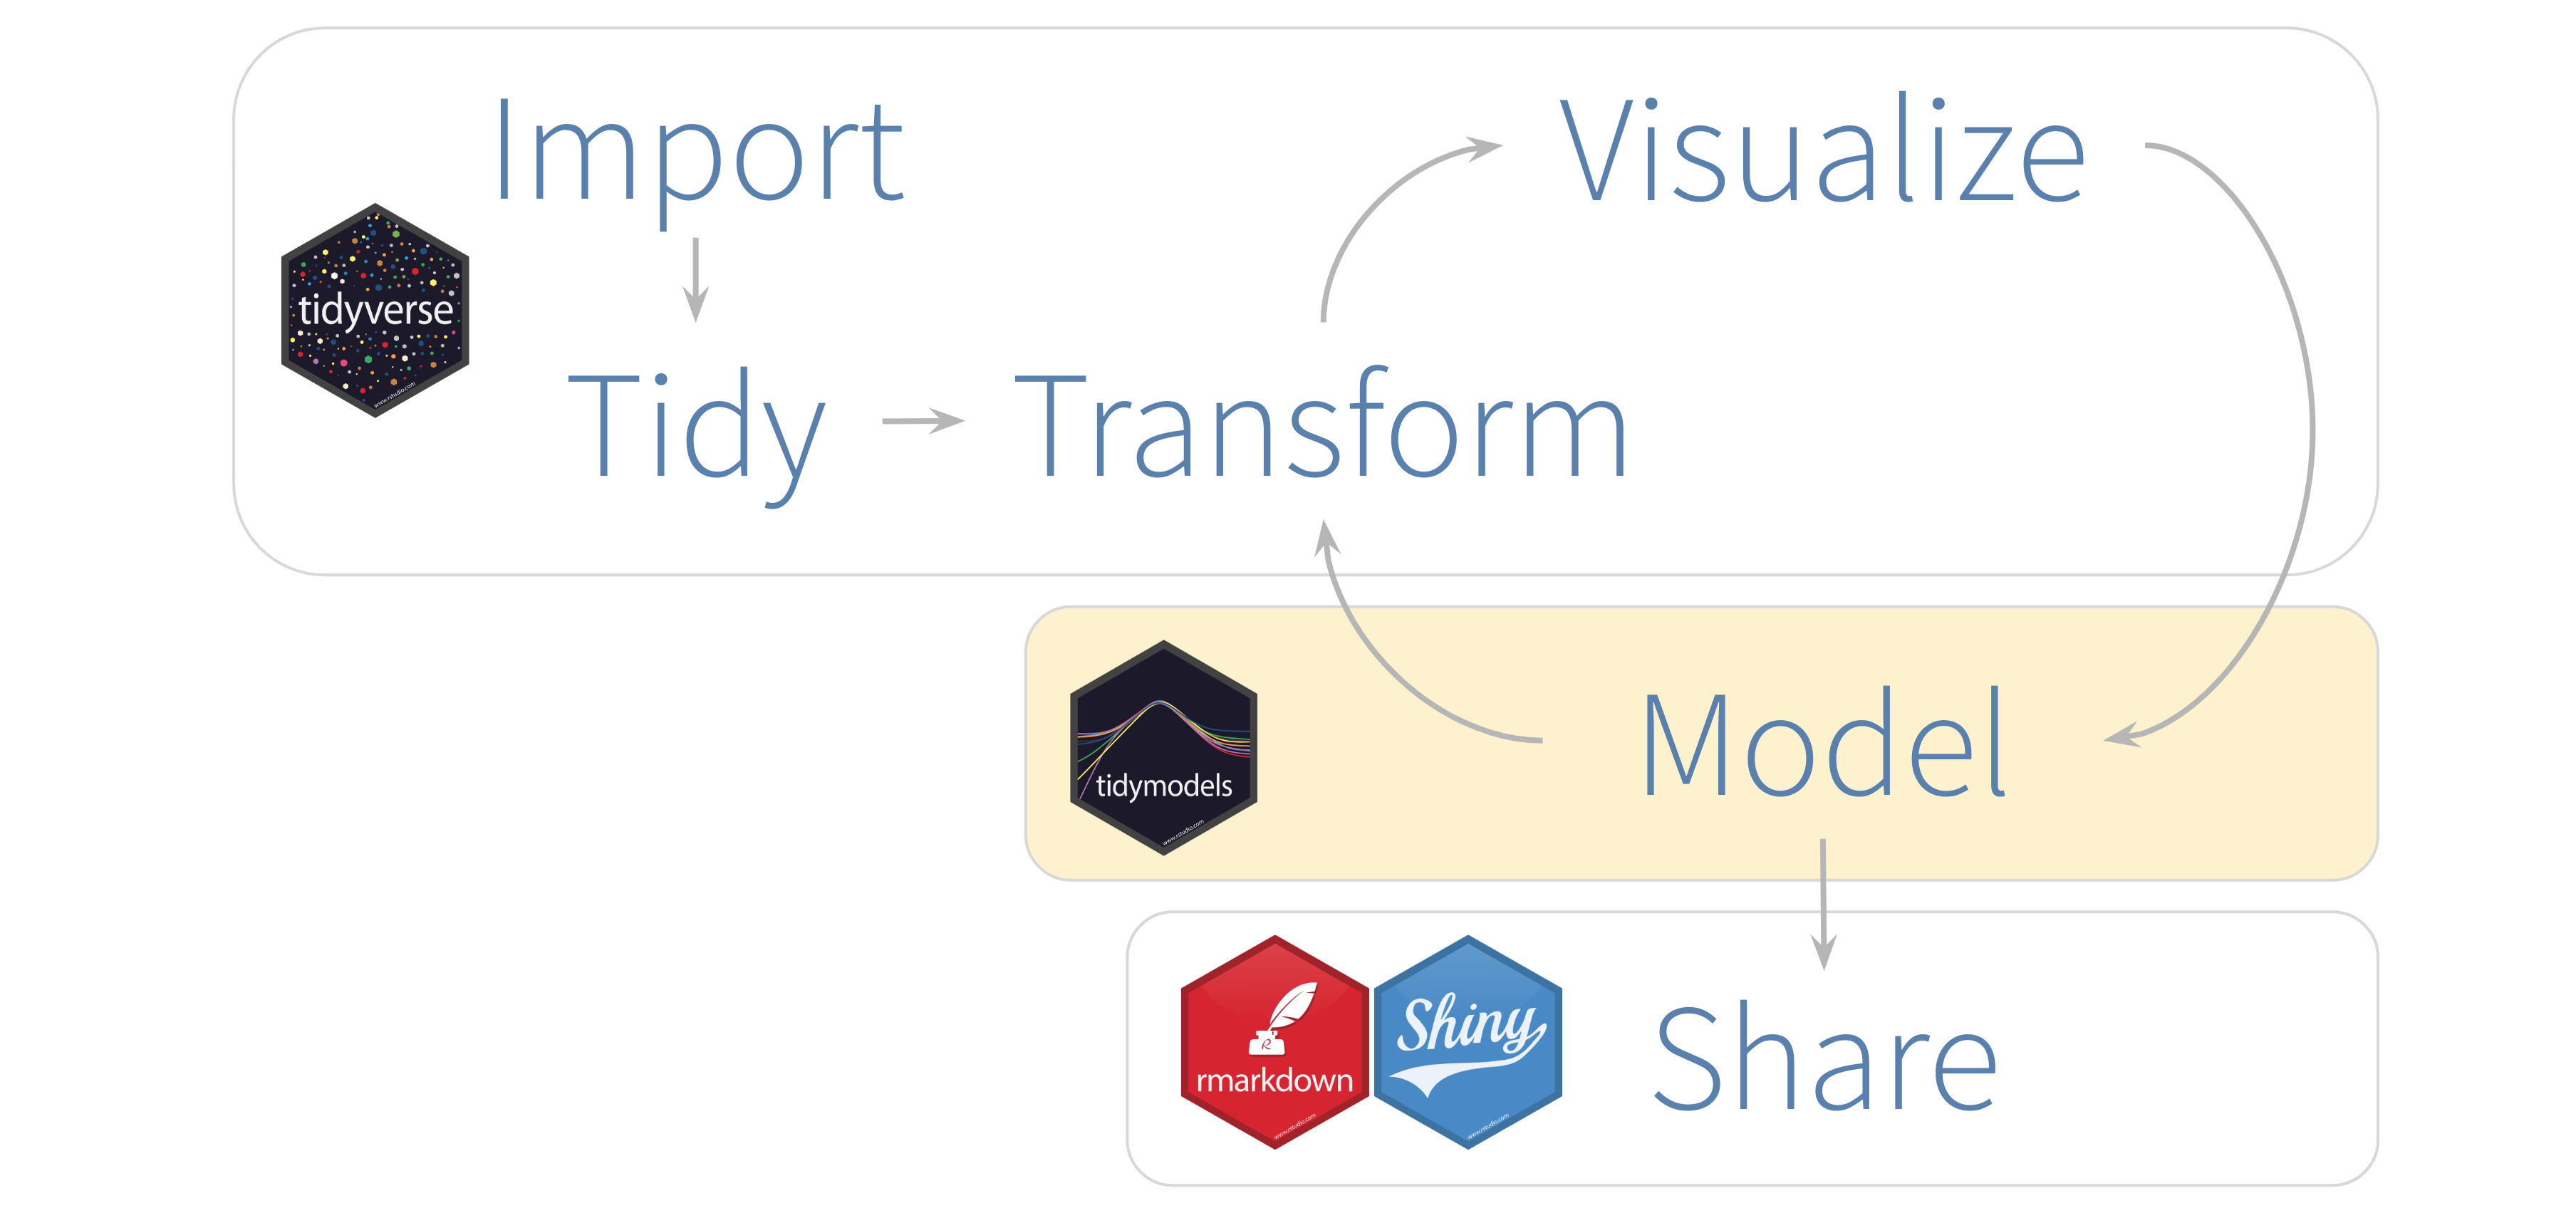
\includegraphics[width=50.22in]{pics/pipeline diagram} *Image taken from
R Views, by Edgar Ruiz\\
This projects aim was to take a simplistic approach at solving customers
propensity to purchase using off the shelf R packages and ML API's with
minimal tuning. Ultimately predictor outcomes will need to be binary,
i.e.~did or did not purchase, and use the applicable ML models. \#\#
Pipeline 1. Data ingestion. R scripts are used to access and down load
zip files from client/banks open web source. 2. Pre-Process and
Re-process. Effectively making the data suitable for modeling and
analysis. This included normalizing field names, bucketing continuous
valuables into discrete chunks, factorizing out outcome variables, and
normalizing numeric predictors to mean zero with standard deviation of
1. This is an iterative step and process that we may return to in order
to reshape our approach. 3. Model and Training. Once again model
selection, training, and tuning is iterative and will be shaped based on
the nature of the questions asked. Here we're asking for a binary, yes
or no, 1 to 0 outcome, so we'll choose a method that addresses those
points first. \#\# Logistic Regression

\end{document}
